\documentclass[preprint]{sig-alternate-05-2015}

\setlength\parindent{0pt}

\usepackage[utf8]{inputenc}
\usepackage[T1]{fontenc}
\usepackage{hyperref}
\usepackage{booktabs}
\usepackage{paralist}
\usepackage{listings,multicol}
\usepackage{lipsum}
\usepackage{cite}
\usepackage{enumerate}
\usepackage{subcaption}
\usepackage{cleveref}
\usepackage{ucs}
\usepackage{framed}

\usepackage[zerostyle=d]{newtxtt}
%\renewcommand*\familydefault{\ttfamily} %% Only if the base font of the document is to be typewriter style
\usepackage[T1]{fontenc}

\usepackage[labelfont=bf]{caption}

\hypersetup{
    colorlinks,
    linkcolor={red!65!black},
    citecolor={blue!50!black},
    urlcolor={blue!80!black}
}

\usepackage{listings}  

\lstset{
	language=PHP,
	basicstyle=\ttfamily\tiny,
	basewidth={0.5em,0.4em}, % for other columns settings
	columns=fullflexible,
	numbers=left,
	numberstyle=\tiny,
	frame=single,
	showstringspaces=false,
	xleftmargin=2em,
	framexleftmargin=1.5em,
	backgroundcolor=\color{lightgrey}
}

\newcommand{\dollar}{\mbox{\textdollar}}


% ARIAL
%\usepackage{helvet}
%\renewcommand{\familydefault}{\sfdefault}


% TIMES
\usepackage{mathptmx}% http://ctan.org/pkg/mathptmx

\usepackage{pgfplots, pgfplotstable}

\usepackage{xcolor}
%\usepackage[dvipsnames]{xcolor}



\definecolor{lightgrey}{HTML}{EEEEEE}

\definecolor{orange}{RGB}{230, 100, 20}
\definecolor{gruen}{RGB}{255, 190, 69}

\definecolor{RYB1}{HTML}{DCDCDC}
\definecolor{RYB2}{HTML}{C0C0C0}
\definecolor{RYB3}{HTML}{808080}

\definecolor{RYB4}{HTML}{DCDCDC}
\definecolor{RYB5}{HTML}{C0C0C0}
\definecolor{RYB6}{HTML}{808080}

\definecolor{RYB7}{HTML}{DCDCDC}
\definecolor{RYB8}{HTML}{C0C0C0}
\definecolor{RYB9}{HTML}{808080}

\definecolor{RYB10}{HTML}{D3D3D3}
\definecolor{RYB11}{HTML}{A9A9A9}

\pgfplotscreateplotcyclelist{ColorListBar}{
{fill=RYB1},
{fill=RYB2},
{fill=RYB3},
}

\pgfplotscreateplotcyclelist{ColorListBar2}{
{fill=RYB4},
{fill=RYB5},
{fill=RYB6},
}

\pgfplotscreateplotcyclelist{ColorListBar3}{
{fill=RYB7},
{fill=RYB8},
{fill=RYB9},
}

\begin{document}
\lstset{
	language=PHP,
	basicstyle=\footnotesize\ttfamily,
    commentstyle = \color{gray},
    extendedchars = \true,
    inputencoding = utf8x,
    keepspaces = true,
    keywordstyle = \bfseries,
    frame = tb
}

% Copyright
\setcopyright{acmcopyright}
%\setcopyright{acmlicensed}
%\setcopyright{rightsretained}
%\setcopyright{usgov}
%\setcopyright{usgovmixed}
%\setcopyright{cagov}
%\setcopyright{cagovmixed}


% DOI
\doi{10.475/123_4}

% ISBN
\isbn{123-4567-24-567/08/06}

%Conference
\conferenceinfo{ISSTA '17}{July 9--13, 2013, Santa Barbara, CA, USA}

\acmPrice{\$15.00}

%
% --- Author Metadata here ---
\conferenceinfo{ISSTA '17}{July 9--13, 2013, Santa Barbara, CA, USA}
%\CopyrightYear{2007} % Allows default copyright year (20XX) to be over-ridden - IF NEED BE.
%\crdata{0-12345-67-8/90/01}  % Allows default copyright data
% (0-89791-88-6/97/05) to be over-ridden - IF NEED BE.
% --- End of Author Metadata ---

\title{Does It Scale? Static Output Approximation of PHP Web Applications Using
Symbolic Execution} 

%


\numberofauthors{3} %  in this sample file, there are a *total*
% of EIGHT authors. SIX appear on the 'first-page' (for formatting
% reasons) and the remaining two appear in the \additionalauthors section.
%
\author{
% You can go ahead and credit any number of authors here,
% e.g. one 'row of three' or two rows (consisting of one row of three
% and a second row of one, two or three).
%
% The command \alignauthor (no curly braces needed) should
% precede each author name, affiliation/snail-mail address and
% e-mail address. Additionally, tag each line of
% affiliation/address with \affaddr, and tag the
% e-mail address with \email.
%
% 1st. author
\alignauthor
Stefan Mühlbauer\\
       \affaddr{TU Braunschweig, Germany}\\
       %\email{s.muehlbauer@tu-bs.de}
% 2nd. author
\alignauthor
Christian Kästner\\
      \affaddr{Carnegie Mellon University, USA}\\
       %\email{ckaestner@cs.cmu.edu}
% 3rd. author
\alignauthor
Tien N. Nguyen\\
       \affaddr{University of Texas, USA}\\
%      %\email{tien.n.nguyen@utdallas.edu}
}
% There's nothing stopping you putting the seventh, eighth, etc.
% author on the opening page (as the 'third row') but we ask,
% for aesthetic reasons that you place these 'additional authors'
% in the \additional authors block, viz.
\additionalauthors{Additional authors: John Smith (The Th{\o}rv{\"a}ld Group,
email: {\texttt{jsmith@affiliation.org}}) and Julius P.~Kumquat
(The Kumquat Consortium, email: {\texttt{jpkumquat@consortium.net}}).}
\date{30 July 1999}
% Just remember to make sure that the TOTAL number of authors
% is the number that will appear on the first page PLUS the
% number that will appear in the \additionalauthors section.

\maketitle
\begin{abstract}
Dynamic web applications have become widely popular and are to
a large proportion based on the scripting language PHP. Output approximation of web
applications enables a range of additional tool support as well as possibilities
for vulnerability detection. Unfortunately, recent approximation approaches have
only been evaluated for smaller systems.

This paper presents an experience report about the scalability of output
approximation using symbolic execution of state-of-the-art PHP web
applications. For a symbolic execution engine extended with support for
object-oriented programming and arrays, we identified language features and
corresponding programming patterns that impede symbolic execution and limit the
scalability of this approach. Our findings include: (1) Dynamic features such as
functions and includes are prone to fail for certain programming patterns. (2)
Expressions containing elements from I/O, databases or files can heavily impede
symbolic execution. Our findings provide useful guidelines to design new
tools and also to improve the development process of statically analyzable web
applications.
\end{abstract}


%
% The code below should be generated by the tool at
% http://dl.acm.org/ccs.cfm
% Please copy and paste the code instead of the example below. 
%
\begin{CCSXML}
<ccs2012>
 <concept>
  <concept_id>10010520.10010553.10010562</concept_id>
  <concept_desc>Computer systems organization~Embedded systems</concept_desc>
  <concept_significance>500</concept_significance>
 </concept>
 <concept>
  <concept_id>10010520.10010575.10010755</concept_id>
  <concept_desc>Computer systems organization~Redundancy</concept_desc>
  <concept_significance>300</concept_significance>
 </concept>
 <concept>
  <concept_id>10010520.10010553.10010554</concept_id>
  <concept_desc>Computer systems organization~Robotics</concept_desc>
  <concept_significance>100</concept_significance>
 </concept>
 <concept>
  <concept_id>10003033.10003083.10003095</concept_id>
  <concept_desc>Networks~Network reliability</concept_desc>
  <concept_significance>100</concept_significance>
 </concept>
</ccs2012>  
\end{CCSXML}

\ccsdesc[500]{Computer systems organization~Embedded systems}
\ccsdesc[300]{Computer systems organization~Redundancy}
\ccsdesc{Computer systems organization~Robotics}
\ccsdesc[100]{Networks~Network reliability}



%
%  Use this command to print the description
%
\printccsdesc

% We no longer use \terms command
%\terms{Theory}

\keywords{Static program behavior, Static metrics, Dynamic language features,
Static Analysis, PHP}

\section{Introduction}
With the emerging world wide web, dynamic web applications have become
widely popular. Various different implementation techniques have emerged,
ranging from technologies for programming languages (JSP, ASP .NET) and web
application frameworks for  script languages (Ruby On Rails, Django) to
languages tailored specifically to the domain of web applications. PHP \cite{phpNET} is
a programming language focused on server-side application development. As of 2012,
it was used by 78.8 percent of the ten million most popular websites (according
to Alexa popularity ranking) \cite{alexaPHP}, ranking 7th on the TIOBE
programming community index \cite{tiobePHP}, and was the ranked as the 6th most
popular language on GitHub \cite{githubPHP}.

One common property of all technologies for dynamic web applications is \emph{staged computation} of output: A dynamic web application as a whole consists of both static code, such as scripts, and dynamically generated code, such as responses to HTTP requests. The latter code, although assembled at runtime, may contain client-side parts of the web application, such as JavaScript. So, to study dynamic web applications in its entirety, we need to consider both static as well as dynamic aspects of systems.

%Since based on both static values and runtime values, output code is generated step by step
%dynamically, output can be dependent on application inputs. Dynamic web
%applications incorporate various both server-side inputs (databases,
%configuration) and client-side inputs respectively. Static
%analysis of dynamic web applications, hence, has to consider different input
%sources.

\emph{Symbolic execution} is a static analysis technique between program testing
and program proving. For a program, symbolic, i.e., abstract, yet fixed inputs are
applied instead of concrete inputs \cite{Darringer1978,King1976}. The underlying
concept is to map program input (symbolically) to program output. Different classes of inputs may
result in variational output, representing dependencies of output and input.
As symbolic execution of a program returns an input-output-mapping for symbolic
inputs, this analysis technique helps unfold the \emph{staged} nature of web
applications: Since every feasible path is executed all possible output is
contained in the symbolic output, and all dynamically generated variational
parts of the web application can be analyzed.

%Symbolic execution extends concrete execution semantics with semantics to
%handle symbolic values. Hence, concrete execution semantics is contained in
%symbolic execution semantics. Symbolic execution has been used and studied for generating test suites, but
%has more recently also been applied for approximating the output of web
%applications. 

Knowledge about different output variants enabled useful analyses
for the domain of web applications, such as detecting and locating HTML
validation errors \cite{Nguyen:2011:AFH:2190078.2190142}. As for developers,
from an output model, outlines and callgraphs for easier IDE code navigation
\cite{Nguyen:2014:BCG:2635868.2635928}, or program slices
\cite{Nguyen:2015:CPS:2786805.2786872} can be computed. Existing work has been
integrated in the Varis plugin for the Eclipse IDE \cite{Nguyen:2015:VIS:2819009.2819140}.

Despite the various use cases for analyses based on an approximated output
model, static output approximation for PHP web applications using symbolic
execution has so far only been evaluated for smaller systems that are not
maintained anymore. The previously mentioned tools though are only practical, if
for a given system the symbolic execution engine is scalable, i.e., will also
approximate output accurately for larger and more recent systems with good time
and space consumption.

To investigate the question, whether we can build practical tools from the
the symbolic execution engine, we re-implemented the engine with the specifications
of the previous symbolic execution semantics
\cite{Nguyen:2014:BCG:2635868.2635928} for PHP and additional features, such as
object-oriented programming. We evaluated our
symbolic execution engine for large-scale and modern PHP systems.

During introduction of new semantics for object-orientation we encountered two
main challenges. First, we were bound to introduce more concrete execution features to the
symbolic execution engine, e.g. foreach loops for arrays, as this increased
code coverage significantly. Second, we had to make a trade-off between the
accuracy of method calls and the scalability of this language feature as a
method call for different program state variants can have multiple targets.

Based on our observations and evaluation results, we learned that for dynamic
PHP constructs, expressions that are assembled dynamically, in combination with
symbolic values symbolic execution can be impractical. For object-orientation
and method calls, symbolic execution semantics can be a tightrope walk between
state space explosion and imprecision. Moreover, the nature of PHP challenges a
practical symbolic execution engine since for it to be accurate, a large number
of functions from the standard library needs to be supported.

Our key contributions in this paper include (1) a new tool infrastructure to
statically approximate the output for PHP web applications using symbolic
execution, and (2) a report of our observations with state-of-the-art web
applications as well as an explanation on conceptual limitations for symbolic
execution of PHP applications.

\section{State Of the Art}\label{sec:stateoftheart}
Symbolic execution is one of integral analysis techniques used by the tools
whose practicality we aim to evaluate. This section recaps the idea of symbolic
execution, the tools which make use of it, and both conceptual and
language-related limitations.

\subsection{Symbolic Execution}
Symbolic execution is a static analysis technique that was proposed by James C.
King in 1976 \cite{King1976}. Symbolic execution allows to explore all feasible
paths in a program. Based on normal program execution, the execution semantics
is extended to handle symbolic values, which are abstract, but fixed; an
execution becomes symbolic by introducing symbolic values as program inputs
instead of concrete values \cite{King1976,Darringer1978}. These symbolic values
are then propagated and used throughout the execution.

Execution starts with a plain path condition, usually a tautology. Whenever the
control-flow can be split into different branches, the corresponding path
conditions (guards for instance) are conjoined with the previous path condition
\cite{King1976}. Additionally, the conjoined path condition can be checked for
satisfiability to exclude infeasible paths. Consequently, for a given program
symbolic execution computes a mapping from (symbolic) input values to output values.

\subsection{Static Output Approximation for PHP} \label{sec:workflow}
Symbolic execution is an analysis technique not dedicated to a particular
programming language. For dynamic web applications, in our case for web
applications written in PHP, it can be used to approximate all possible client
page output. Before we present in detail existing tools that aim to ease
development and maintenance of PHP web applications, we illustrate how output
approximation using symbolic execution is used by starting with an example.

\begin{figure}[t]
	\centering
	\begin{subfigure}[center]{0.48\textwidth}%%[multicols=1]
\begin{lstlisting}
<form>
  <input type="text" name="name">
  <input type="submit" value="Submit">
</form>

<?php
function make_titles($arg, $n) {
  $is = shuffle(array(1,2,3));
  while ($n < $is[0]) {
    echo "<h1>" . $arg . "</h1><br />";
    $n = $n + 1;
  }
}
  
call_user_func("make_titles", "Headline", 4);

$greeting = "Hello " . $_POST['name'] .  "!";
if (!isset($_POST['name'])) {
  echo "No name entered!";
} else {
  echo $greeting;
}
?>
\end{lstlisting}
		\caption{Snippet of HTML and PHP server-side web application code.
		\label{fig:web_application}}
    \end{subfigure}

	\vspace{2mm}    
    
    ~ %add desired spacing between images, e. g. ~, \quad, \qquad, \hfill etc. 
      %(or a blank line to force the subfigure onto a new line)
    \begin{subfigure}[center]{0.48\textwidth}
\begin{lstlisting}[mathescape]
<form>
  <input type="text" name="name">
  <input type="submit" value="Submit">
</form>

// #repeat n < shuffle(is)
<h1>Headline</h1><br />
// #endrepeat

// #if !isset(name)
No name entered!
// #else
Entered $\alpha$!
// #endif

\end{lstlisting}
		\caption{
			Approximation client paege output of the server-side web application code in
			Figure \ref{fig:web_application}. Variability as well as repetition annotations
			are represented by preprocessor directives.
			\label{fig:output_example}
		}
    \end{subfigure}
    \vspace{2mm}
    \caption{
    	Illustration of static ouptut approximation using symbolic
    	execution
    	\label{fig:code_example}
    }
\end{figure}

Figure \ref{fig:code_example} shows two code listings. The snippet of server-side web
application code in Figure \ref{fig:web_application} contains both HTML and PHP. First, the
function \texttt{make\_titles} defined in lines 7 – 13 prints the string
\texttt{\$arg} passed as an argument between zero and an arbitrary number of
times. Second, the function is indirectly called using the built-in function
\texttt{call\_user\_func} in line 15 with the string \texttt{Headline} and
\texttt{4} as arguments.  Finally, the input from the form in lines 1 – 4 is
used: The variable \texttt{\$greeting} consists of three concatenated strings,
\texttt{Hello} the value of input field \texttt{name}, and an exclamation mark.
For this server-side code snippet there are two possible client page output
variants: If the input field \texttt{name} is empty at runtime, line 19 is
executed and \texttt{No name entered!} is printed, or, if a name was entered,
line 21 is executed and the greeting constructed in line 17 is printed.



%C. Introduction to symbolic execution of PHP code
The following symbolic execution semantics for PHP features  based on \cite{Nguyen:2014:BCG:2635868.2635928}
illustrate the necessary modifications made to handle the extent of ambiguity
that comes with handling symbolic values. In addition to normal output, the
output approximation contains preprocessor directives to express
repeatable output as well as output variants. All approximated client page
output corresponding to Figure \ref{fig:web_application} consisting of two different variants
is illustrated in Figure \ref{fig:output_example}.
First, loops in the previous execution semantics are only executed once instead
of an arbitrary number of times. Since a loop condition can contain symbolic
values, it might not be feasible to determine when a loop terminates. Hence,
any output constructed during the single loop iteration is highlighted
(\texttt{repeat \ldots  endrepeat}) to possibly be repeated an arbitrary number
of times. The output in line 7 is marked to be repeated an arbitrary number of times, as the number
of loop iterations cannot be determined statically. Second, a similar procedure
applies to recursive functions. Once called, a recursive function is  also only
executed to recursion depth one per call, and any subsequent invocation of that
function returns a symbolic value. This, again, is due to the difficulty to
determine the exact recursion depth similar to the number of loop iterations.
Third, since the symbolic execution engine applies a static analysis, any form
of user interaction providing input data as well as any form of input referred
to from the deployment context of the web application, i.e. configuration files
or databases, is substituted by a symbolic value. The context variable
\texttt{\$\_POST} represents input submitted to the server and, hence, is
symbolic as every program input is per definition substituted by symbolic values. Finally, the
output in lines 11 and 13 respectively are marked as alternatives
(\texttt{if \ldots else \ldots endif}), as symbolic execution of lines 18 – 22
in Figure \ref{fig:web_application} will explore both different branches.

\subsection{Existing Tool Support for PHP}
All tools proposed so far leverage a representation of all possible HTML client
page output. Since any variant can be analyzed in particular, this enables tool
support addressing the web application as a whole in spite of its staged
nature, where parts of the web application (client-side output) are generated
dynamically.

Based on the approximated output representation subsequent analyses can be
conducted, which have been implemented in the following tools:

\begin{compactitem}
	\item \emph{PhpSync}: Using all variants of  HTML client page output, every
	single one can be statically checked for Markup Validity, i.e., if the web page
	conforms to syntactical specifications for HTML and other client-side
	languages. After validation errors are detected, auto-fixes are provided.
	Otherwise, the validation error can be traced back to source code responsible
	for the defect, which then can be refactored manually
	\cite{Nguyen:2011:AFH:2190078.2190142}.

	\item \emph{WebSlice}: Program slices enable to extract and understand the
	impact of changes in an application. To consider all of a dynamic web
	application for program slices, client page output needs to be taken into
	account. WebSlice combines PHP data-flow information with an output
	approximation to enable program slices across different languages
	\cite{Nguyen:2015:CPS:2786805.2786872}.

	\item \emph{Varis}: Editor services such as “jump to declaration” are
	nontrivial for dynamic web applications due to their staged nature. Varis
	provides editor services across stages for client-side code: Starting with an
	ouput approximation a callgraph with conditional edges is constructed, which
	allows navigation in client-site code (HTML, JS and CSS) although it is
	embedded in server-side code
	\cite{Nguyen:2015:VIS:2819009.2819140,Nguyen:2014:BCG:2635868.2635928}.
\end{compactitem}

All three tools though have only been applied to systems that are small and not
maintained any more. Despite the functional benefits these tools provide to
developers, their practicality for large and modern systems has not been
studied.

%\subsection{Assumptions and Limitations}
%Symbolic execution remains an analysis technique not dedicated to a particular programming language. For the implementation of the symbolic execution engine in \cite{Nguyen:2014:BCG:2635868.2635928,Nguyen:2015:CPS:2786805.2786872}, several assumptions have been made to adapt to the PHP language. The following symbolic execution semantics for PHP features differ from concrete execution since symbolic values need to be handled without ambiguity. 

%First, loops in the previous execution semantics are only executed once instead of an arbitrary number of times. Since a loop condition can contain symbolic values, it might not be feasible to determine when a loop terminates. Hence, any output constructed during the single loop iteration is highlighted to possibly be repeated  an arbitrary number of times. Second, recursive functions are also only executed once per call, and any subsequent call ot that function returns a symbolic value. This, again, is due to the difficulty to determine the exact recursion depth similar to the number of loop iterations. Finally, since the symbolic execution engine applies a static analysis, any form of user interaction providing input data as well as any form of input referred to from the deployment context of the web application, i.e. configuration files or databases, is substituted by a symbolic value. 

%Language-wise the symbolic execution semantics for the tools presented in Section \ref{sec:workflow} currently does not support object-oriented programming. PHP provides a large number of built-in functions to manipulate strings as well as arrays. The current symbolic execution engine only provides implementations for a small range of PHP standard library functions, mainly string operations. 

\section{Scalable Output Approximation}%
The main objective of this experience report is to investigate whether the
tools described in Section \ref{sec:stateoftheart} are practical. In particular
we want to find out whether symbolic execution as the underlying technique for
static output approximation scales for PHP, and what may limitations restrict
scalability. We may divide possible limitations into either matters of
engineering or conceptual limitations where no precise execution is possible.

In the following we describe in detail our implementation procedure, practical
problems we encountered and whether these are limiting scalability conceptually
or just require en gineering effort to be tamed.

\subsection{Towards Scalable Output Approximation?}
We re-implement\footnote{\url{https://github.com/smba/oak}} the existing
symbolic execution semantics of \cite{Nguyen:2014:BCG:2635868.2635928} with the
goal to support modern large-scale dynamic web applications, or at least to
better understand possible limitations. For reference, we choose to aim to
support  \textsf{WordPress}
\footnote{\url{https://github.com/WordPress/WordPress }}, a popular Content
Management System of reasonable size that is still maintained. Moreover, our
implementation uses parts of
Quercus\footnote{\url{http://quercus.caucho.com/}}, a pure Java implementation
of the PHP interpreter, which is tested against the \textsf{WordPress} test
suite. We choose a test-driven approach for our implementation with regression
tests and continuous integration. Our test cases are based on both custom
examples for different language features as well as \textsf{SchoolMate}, a 
small-scale system, and, at least in parts, \textsf{WordPress}, whose output we
manually validate and then automatically re-check for each test run.

Our implementation basically follows the symbolic execution semantics of
\cite{Nguyen:2014:BCG:2635868.2635928}, yet we extend it with additional rules
for class definitions, class instantiation, and method invocation to support
object-oriented programming. Furthermore, we add rules for do-while and 
foreach loops since these are not supported as yet. Note that we execute all
iterations of a foreach loop since the number of iterations is known since we
 are traversing all items of a given array.

 \section{Evaluation}
As already stated in the previous section, we encountered sevaral problems
during the development of the symbolic interpreter. Therefore this section
describes our methods to evaluate practicality of the output approximation, and
possible explanations.

\subsection{Measuring Approximation Success} \label{heuristic}
For the evaluation of our output approximation we require a ground truth output
model to compare our approximation against. Since output literals are embedded
in server-side code and scattered, it is nontrivial to determine whether a
string literal is part of the ouput or not. So, in the absence of ground truth
for the approximated output we are bound to choose a \emph{heuristic approach}
in order to measure the accuracy of our aproximation. We define a string
literal to be an \emph{output candidate} if there exists an execution path
reaching the string literal and evantually passing it to an output-generating
statement (e.g., \texttt{echo} or \texttt{print}).

We approximate output candidates as those string literals containing the
characters \texttt{<}, \texttt{>}, or both since we expect output to contain
HTML tags. We evaluated this heuristic manually with a sample of 400 string
literals randomly selected from the entire corpus.
We measured for our heuristic classifier a precision of 94 percent, and a
recall of 50 percent. This means that six percent of the string literals are
classified incorrectly as false positives. In turn, the classifier is highly
distinctive as 96 percent of the string literals are classified correctly. The
recall of 50 percent means that half of the string literals, which we manually 
classified as output, actually were responsive to the classifier. We attempted
to increase recall by looking for further distinctive properties to build a
classifier from, but could not do so without decreasing precision. In spite of
missing half of the output candidates, we decided to use a simple, yet
distinctive classifier.

\subsection{Experiment Setup} 
For the evaluation we symbolically executed a selection of PHP systems. We
selected a corpus of twelve PHP systems with regard to system size and recency
as the corpus of the case study for \cite{Nguyen:2014:BCG:2635868.2635928} only
contained small-scale systems that are not maintained any more. The full list
of PHP systems is shown in Table \ref{corpus}. Our selection of PHP systems
includes

%
\begin{compactitem}
	\item four small-scale systems that selected from the previously mentioned case
	study in order to compare our results with the previous symbolic execution
	engine \cite{Nguyen:2014:BCG:2635868.2635928},

	\item three recent large-scale systems selected from the case study corpus of
	\cite{Hills:2013:ESP:2483760.2483786}, and
	
	\item four small-scale systems selected from a list of recent Content
	Management Systems \cite{codegeekz}.
\end{compactitem}

As for for the last two cases, we limited our selection since the parser we
used did not support all language features used. For the experimental evaluation we symbolically executed per system each script file or entry point (files with a \texttt{.php}, \texttt{.inc}, \texttt{.bit} or \texttt{.module} extension). All following measurements are cumulated per system for each entry point. 

\begin{table*}[t]
\centering 
	\begin{tabular}{lrp{4cm}rrrr}
	\toprule
	\textbf{System} & \textbf{Version} & \textbf{Classification} & \textbf{SLOC} &
	\textbf{\#files} & \textbf{\#OCs} & \textbf{\#includes}
	\\
	\midrule
	AddressBook & 8.2.5.2 &  & 51,907 & 239  & 1009 & 186\\
	SchoolMate & 1.5.4 &  & 8,118 & 65  & 853 & 88\\
	TimeClock & 1.04 &  & 20,800 & 63  & 7920 & 306\\
	WebChess & 1.0.0 &  & 5,219 & 28  & 470 & 56\\
	\midrule
	Drupal & 7.5.0 & CMS & 52,464 & 125  & 3569 & 749\\
	phpBB & 3.1.9 &  & 327,371 & 1,398  & 3606 & 206\\
	phpMyAdmin & 4.6.3 &  & 303,582 & 871  & 7103 & 571\\
	\midrule
	Anchor & 0.12.1 &  & 15,054 & 201 & 987 & 32\\
	Kirby & XXX & CMS & XXX & XXX  & 654 & 23\\
	Automad & XXX & CMS & XXX & XXX  & 655 & 8\\
	Monstra & XXX & CMS & XXX & XXX  & 1934 & 48\\
	Nibbleblog & XXX & CMS & XXX & XXX  & 1013 & 28\\
	\bottomrule
	\end{tabular}
	\caption{Corpus of twelve PHP systems. The file count includes files with a .php,
	.inc, .bit or .module extension.}
	\label{corpus}
\end{table*}


\subsection{Measuring Approximation Accuracy}
\label{HowAccurateIsOurApproximation} 
In Section \ref{heuristic} we introduced the definition of output candidates as
expected output. As a most accurate approximation contains all output
candidates, we define two metrics to measure accuracy of our approximation.

First, we measure how much of the expected output was actually processed by the
symbolic interpreter.  Once a line of code, a statement or expression
containing an output candidate is actually an element in an execution path, we
define this output candidate as reached. We define the metric \emph{reach
coverage} as the ratio of output candidates that are reached and the total
number of output candidates in the analyzed system. Although a reached output
candidate is processed by the symbolic interpreter, it does not guarantee we
will see that output candidate in the symbolic output. Second, we define the
metric \emph{output coverage} as the ratio of output candidates that are
contained in the output of the symbolic interpreter and the total number of
output candidates in the analyzed system.  For an imprecise approximation, we
may see loss of output candidate information resulting in a output coverage
lower than the reach coverage.

The coverage results are illustrated in Figure \ref{coverage}. We could
replicate high coverage results for the four small-scale systems with a reach
coverage and output coverage over 80 percent respectively. For the three
modern/large-scale systems we measured poor coverage with reach coverage
ranging from 5 to 30 percent and output coverage ranging from 4 to 20 percent.
We measured medium to high coverage for the more recent small-scale systems:
reach coverage ranging from 43 to 85 percent, output coverage ranging from 40
to 85 percent.

\subsection{Understanding Limitations}
As we have seen in Section \ref{HowAccurateIsOurApproximation} both measured
coverage metrics were poor for large-scale and small-scale/recent systems. To
understand what output candidates we missed and why, we further investigated
our approximation results and conducted three more measurements.

\subsubsection{What literals did we miss?}\label{WhatLiteralsDidWeMiss?}
Our initial approach to understand missed output candidates is to find out
whether their surrounding program code was not accessed/accessible, and if so,
why. Of special interest are those output candidates that are located in HTML
files (possibly with nested PHP), or located in a function definition. Plain
HTML files do not require any further execution (of course, unless PHP scripts
are embedded) and represent output candidates that just need to be included
properly to be part of the output. Aside, output candidates that are part of a
function definition are only missed if the corresponding function is never
called at runtime.

We started classifying missed output candidates by their string literal
context. As the classification statistics in Figure \ref{coverage} illustrate,
for almost all systems (except for \textsf{AddressBook} and \textsf{TimeClock})
not-reached output candidates had a function context. Note that
\textsf{SchoolMate} was excluded from the diagram since our analysis reached
all output candidates for that system.

\subsubsection{Inaccessible Dynamic Features}
\label{sec:inaccessible}
For both cases of context, either inclusion of a script file failed, or a
function call failed. If an HTML file is not part of the output, it also is
never reached, i.e., included. An include can fail due to various reasons, such
as an imprecise evaluation of the include expression returning a symbolic
value, or simply a missing file.

For a function to be never reached there are several scenarios: A function is
undefined at runtime if the corresponding script file is never included. In
turn, if the function is defined at runtime the function can either be dead
code if there is no call site for this function, or the function call failed.
In PHP there are several ways to call a function beside direct call sites. The
language offers indirect call mechanisms like callback-commands or an
evaluation function that parses and evaluates PHP source code as strings.

Given a symbolic value, indirect call mechanisms like callback-commands are
likely to fail since target function name and the symbolic value do not match.
This also applies for the evaluation of include expressions as concrete values
representing include targets can be included, but any include target containing
symbolic values is ambiguous.

\subsubsection{Why did includes fail?}
\label{WhyDidIncludesFail}
To better understand include expression evaluation, we use another metric to
approach accuracy from a different angle: We measure (1) the ratio of reached
include expressions and the total number of include expressions in a system
respectively (coverage of include expressions), and (2) the ratio of
successfully resolved include expressions and reached include expressions in a
system (resolution success rate). For a most accurate result all include
expressions are reached and resolved.

For include expressions we sampled failed attempts and manually evaluated the
cause of failure. We identified for (1) that all failed attempts were dynamic
include expressions, i.e., those which were resolved at runtime and were
assembled from fragments of environment-dependent information including
database retrievals, user input, or files. Consequently, the resolved include
expressions contained symbolic values which did not represent identifiable
script files.

Finally, we measured for include expressions the overall reach coverage and the
overall resolution success rate per system. As illustrated in Figure
\ref{fig:include_coverage_results}, except for the small-scale systems and two
recent small-scale systems we did not even really reach a great portion of
include expressions, although for most systems the resolution success rate was
over 80 percent. Nevertheless, one failed attempt to include a script file can
result in a cascade of missing more include expressions as the include target
script is not executed.

\subsubsection{Why did function calls fail?}
\label{WhyDidFunctionCallsFail}
Aside from failed or successful includes, this metric describes one scenario of
why functions containing not-reached output candidates are never called: The
trivial explanation would be that there are no direct calls of those functions,
yet PHP offers a number of ways to call a function indirectly, for instance
using built-in functions, or simply evaluating strings as PHP code using the
\texttt{eval} function.

Moreover we need to take into account that one missed function execution can
result in missing even more function calls (direct or indirect) and executions.
Thus, for functions containing not-reached output candidates we measure whether
they can be (1) only, (2) partially or (3) never accessed transitively from
functions that have no direct call sites. We refer to those functions (or
access points) having no direct call site as callback candidates since the only
way to reach them is through indirect mechanisms. Measuring how many
not-reached output candidates can be explained by functions that are callback
candidates helps to understand whether, and if so, indirect call mechanisms and
their usage may impact our analysis’ code coverage.

The callgraph snippets in Figure \ref{fig:callgraph} illustrate the idea of
detecting the functions’ access points: The nodes at the top depict callback
candidates, the nodes at the bottom with labels X, Y, and Z depict function
definitions containing not-reached output candidates. In Figure
\ref{fig:callgraph} function X can only be accessed through callback
candidates, as for Figure \ref{fig:callgraph} function Y can be partially
accessed by callback candidates, whereas function Z is never accessible through
callback candidates.

% Callback candidate description
\begin{figure}[t!]
	%\centering
	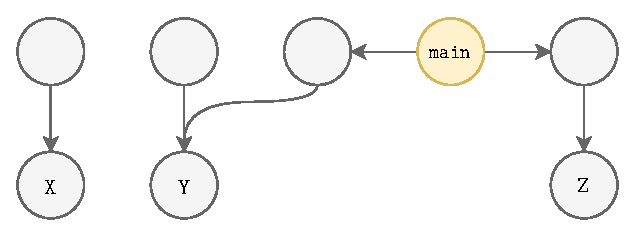
\includegraphics[scale=0.55]{images-paper/callgraph_cases}
    \caption{Callgraph analysis: The bottom nodes represent functions containing missed output candidates, the top nodes depict entry points to them.}
    \label{fig:callgraph} output candidates we measured how many of those functions were only, or partially accessibly through indirect calling mechanisms (see Section \ref{sec:inaccessible}). As Figure \ref{fig:output_candidate_explanation} illustrates, around 80 percent (except for \textsf{TimeClock}) all missed output candidates of each system were only accessible through callback candidates, i.e., functions that are only accessible through indirect calling mechanisms.
	
\end{figure}

Like for include expressions, we again sampled dead function cases and
identified the lack of direct call sites to those functions. As described in
Section \ref{sec:inaccessible}, functions despite having no direct call sites
were called through indirect call features. We identified dynamically assembled
expressions (function names) to be responsible for failed attempts of calling a
function indirectly as the resolved function name eventually contained symbolic
values. These expressions, as well as include expressions, contained
information dependent on the system environment.

For failed function calls to functions containing not-reached
	
	
	% RESULT DIAGRAMS
\begin{figure}[h!]
	\begin{subfigure}[center]{0.48\textwidth}
		\definecolor{bener1}{HTML}{a0c8a0}
\definecolor{bener2}{HTML}{CFC990}
\definecolor{bener3}{HTML}{FFFF99}
\definecolor{bener4}{HTML}{CCCCCC}
\definecolor{bener5}{HTML}{000000}

\pgfplotstableread{ % data 
Label     Reached/Output OnlyReached FunctionContext NotImported Misc
Nibbleblog      59  12  26  0   3
Monstra         61  18  17  0   3
Automad         40  7   49  0   4
Kirby           76  0   23  1   0
Anchor          90  1   10  0   0
phpMyAdmin      4   1   87  1   7
Drupal          18  2   80  0   0
PhpBB           5   27  66  0   3
Webchess        89  3   7   0   1
Timeclock       91  1   0   0   8
Schoolmate      98  2   0   0   0
Adressbook      84  2   4   1   9
    }\testdata

\begin{center}
    \begin{tikzpicture}[thick,scale=0.7, every node/.style={transform shape}]

    \begin{axis}[
    enlargelimits=0.05,
    xbar stacked,   % Stacked horizontal bars
    xlabel={Proportion [\%]},
    xmin=0,         % Start x axis at 0
    ytick=data,     % Use as many tick labels as y coordinates
    legend style={
       at={(1.3, 0.9)}, 
       anchor=north,
       legend columns = 1,
       cells={anchor=center, fill},
       nodes={inner sep=1.5,below=-1.1ex}
    },
    yticklabels from table={\testdata}{Label}  % Get the labels from the Label
    % column of the \datatable
    ,bar width=2ex, y=3ex,
    nodes near coords = {%
       \pgfmathprintnumberto[fixed,assume math mode=true]{\pgfplotspointmeta}{\myval}%
       \pgfmathparse{\myval<101?:}\pgfmathresult%
    },
    area legend
    ]
    
    \addplot +[
    	black,
    	fill=white,
    	postaction={
        pattern=crosshatch%north east lines
    }] table [
    	x=Reached/Output, 
    	meta=Label,
    	y expr=\coordindex
    ] {\testdata}; 
    
    \addplot +[
    	black,
    	fill=white,
    	postaction={
        pattern=north east lines
    }] table [
    	x=OnlyReached, 
    	meta=Label,
    	y expr=\coordindex
    ]    {\testdata}; 
    
    \addplot [fill=white!100] table [
    	x=FunctionContext, 
    	meta=Label,
    	y expr=\coordindex
    ] {\testdata};
     
    \addplot [fill=bener4!100] table [
    	x=NotImported, 
    	meta=Label,
    	y expr=\coordindex
    ] {\testdata};    
    
	\addplot [fill=bener5!100] table [
		x=Misc, 
		meta=Label,
		y expr=\coordindex
	] {\testdata}; \
	    
    \legend{Reached/Output, OnlyReached, FunctionContext, NotImported, Misc}
    \end{axis}
    \end{tikzpicture}
 \end{center}
		\caption{\label{coverage}}
	\end{subfigure}
	
	\begin{subfigure}[center]{0.48\textwidth}
		\definecolor{bena1}{HTML}{a0c8a0}
\definecolor{bena2}{HTML}{CFC990}
\definecolor{bena3}{HTML}{CCCCCC}

\pgfplotstableread{ % data 
Label	Reached/Resolved  OnlyReached NotReached
Adressbook	92	4	3
Schoolmate	100	0	0
Timeclock	92	0	8
Webchess	95	0	5
PhpBB	48	17	35
Drupal	43	6	51
phpMyAdmin	39	0	60
Anchor	0	84	16
Kirby	0	39	61
Automad	38	0	63
Monstra	10	27	63
Nibbleblog	91	9	0

    }\testdata

\begin{center}
    \begin{tikzpicture}[thick,scale=0.6, every node/.style={transform shape}]

    \begin{axis}[
    enlargelimits=0.05,
    xbar stacked,   % Stacked horizontal bars
    xlabel={Proportion [\%]},
    xmin=0,         % Start x axis at 0
    ytick=data,     % Use as many tick labels as y coordinates
    legend style={
       at={(1.3, 0.9)}, 
       anchor=north,
       legend columns = 1,
       cells={anchor=center, fill},
       nodes={inner sep=1.5,below=-1.1ex}
    },
    yticklabels from table={\testdata}{Label}  % Get the labels from the Label column of the \datatable
    ,bar width=2ex, y=3ex,
    nodes near coords = {%
       \pgfmathprintnumberto[fixed,assume math mode=true]{\pgfplotspointmeta}{\myval}%
       \pgfmathparse{\myval<101?:}\pgfmathresult%
    },
    area legend
    ]
    
    \addplot [fill=bena1!100] table [
    	x=Reached/Resolved, 
    	meta=Label,
    	y expr=\coordindex
    ] {\testdata}; 
    
    \addplot [fill=bena2!100] table [
    	x=OnlyReached, 
    	meta=Label,
    	y expr=\coordindex
    ]    {\testdata}; 
    
    \addplot [fill=bena3!100] table [
    	x=NotReached, 
    	meta=Label,
    	y expr=\coordindex
    ] {\testdata};
     
    \legend{Reached/Resolved, OnlyReached, NotReached}
    \end{axis}
    \end{tikzpicture}
 \end{center}
		\caption{
			Include coverage and accuracy.
			\label{fig:include_coverage_results}
		}
	\end{subfigure}
	
	
	% Callback candidate explanation
	\begin{subfigure}[center]{0.48\textwidth}
		\definecolor{bene1}{HTML}{a0c8a0}
\definecolor{bene2}{HTML}{CFC990}
\definecolor{bene3}{HTML}{CCCCCC}

\pgfplotstableread{ % data 
Label	Complete  Partial Not
Nibbleblog  100     0       0
Monstra     100     0       0
Automad     100     0       0
Kirby       98      1       1
Anchor      79      3       18
phpMyAdmin  99      0       0
Drupal      87      3       10
PhpBB       94      1       5
Webchess    79      0       21
Timeclock   0       0       100
Schoolmate  0       0       100
Adressbook  100     0       0

    }\testdata

\begin{center}
    \begin{tikzpicture}[thick,scale=0.7, every node/.style={transform shape}]

    \begin{axis}[
    enlargelimits=0.05,
    xbar stacked,   % Stacked horizontal bars
    xlabel={Proportion [\%]},
    xmin=0,         % Start x axis at 0
    ytick=data,     % Use as many tick labels as y coordinates
    legend style={
       at={(1.3, 0.9)}, 
       anchor=north,
       legend columns = 1,
       cells={anchor=center, fill},
       nodes={inner sep=1.5,below=-1.1ex}
    },
    yticklabels from table={\testdata}{Label}  % Get the labels from the Label column of the \datatable
    ,bar width=2ex, y=3ex,
    nodes near coords = {%
       \pgfmathprintnumberto[fixed,assume math mode=true]{\pgfplotspointmeta}{\myval}%
       \pgfmathparse{\myval<101?:}\pgfmathresult%
    },
    area legend
    ]
    
    \addplot +[
    	black,
    	fill=white,
    	postaction={
        pattern=crosshatch%north east lines
    }] table [
    	x=Complete, 
    	meta=Label,
    	y expr=\coordindex
    ] {\testdata}; 
    
    \addplot +[
    	black,
    	fill=white,
    	postaction={
        pattern=north east lines
    }] table [
    	x=Partial, 
    	meta=Label,
    	y expr=\coordindex
    ]    {\testdata}; 
    
    \addplot [fill=white!100] table [
    	x=Not, 
    	meta=Label,
    	y expr=\coordindex
    ] {\testdata};
     
    \legend{Complete, Partial, Not}
    \end{axis}
    \end{tikzpicture}
 \end{center}
		\caption{
			Distribution dead function output candidates that are par-
			tially or completely explained due to callback candidates.
			\label{fig:output_candidate_explanation}
		}
		
	\end{subfigure}
	\caption{Results}
\end{figure}
\section{Lessons Learned}

\section{Related Work}
\begin{itemize}
	\item Hills et al. \cite{Hills:2013:ESP:2483760.2483786}
	\item Output approximation using context-free grammar construction; applications \cite{minamide2005static,wassermann2007sound}
\end{itemize}

%References
\bibliographystyle{abbrv}
\bibliography{bibliography}

\end{document}
